\documentclass[twoside, openright, 12pt]{book}
\usepackage{fourier}
%\usepackage{tkz-berge}
%\usepackage{amsmath, amsthm, amssymb}
\usepackage{amsmath, amssymb}
\usepackage{enumerate, url, verbatim, sagetex}
\usepackage{hyperref}% wants to be last

\pagestyle{headings}

% \newtheoremstyle{plainsl}%
% 	{\topsep}
% 	{\topsep}
% 	{\slshape} % only non-default setting
% 	{}
% 	{\normalfont\bfseries}
% 	{.}
% 	{ }
% 	{}
% 
% % I prefer 1.2 Lemma to Lemma 1.2
% \swapnumbers
% 
% \theoremstyle{plainsl}
% \newtheorem{theorem}{Theorem}[section]
% \newtheorem{lemma}[theorem]{Lemma}
% \newtheorem{corollary}[theorem]{Corollary}
% 
% % I label my lemmas with tags of the form lem:name,
% % and then I cite them as \lref{name}; you might not want to bother
% \newcommand\chref[1]{Chapter~\ref{cha:#1}}
% \newcommand\lref[1]{Lemma~\ref{lem:#1}}
% \newcommand\tref[1]{Theorem~\ref{thm:#1}}
% \newcommand\cref[1]{Corollary~\ref{cor:#1}}
% \newcommand\sref[1]{Section~\ref{sec:#1}}
% 
% % I do not like the ams proof environment, because it inserts too much
% % space between the statement of the theorem/lemma/whatever and the proof
% % so I use \proof text.\qed
% % The AMS proof environment will not function properly once \proof
% % and \qed are defined as below.
% % If you want the default AMS theorem style, replace \textsl by \texit on the next line.
% \renewcommand\proof{\noindent\textsl{Proof. }}
% \newcommand\sqr[2]{{\vbox{\hrule height.#2pt
%     \hbox{\vrule width.#2pt height#1pt \kern#1pt
%         \vrule width.#2pt}\hrule height.#2pt}}}
% % Put \qed at the end of each proof, flush against the full stop.
% \renewcommand\qed{%
% 	\ifmmode\eqno\sqr53
% 	\else\nolinebreak\ \hfill\sqr53\medbreak\fi}
% 
% %% end of theorem/proof adjustments %%%%%%%%%%%%%%%%%%%%%%%%%%%

%% equation numbers in each section start at 1,
%% references to equation numbers should include the section, of course
\numberwithin{equation}{section}

\newcommand\al{\alpha}
\newcommand\be{\beta}
\newcommand\de{\delta}
\newcommand\De{\Delta}
\newcommand\eps{\epsilon}
\newcommand\ga{\gamma}
\newcommand\Ga{\Gamma}
\newcommand\ka{\kappa}
\newcommand\la{\lambda}
\newcommand\La{\Lambda}
\newcommand\om{\omega}
\newcommand\Om{\Omega}
\newcommand\sg{\sigma}
\newcommand\Sg{\Sigma}
\renewcommand\th{\theta} %--- Latex uses \th for a Norse character
\newcommand\Th{\Theta}
\newcommand\vphi{\varphi}

%
% some calligraphy
%
\newcommand\cA{{\mathcal A}}
\newcommand\cB{{\mathcal B}}
\newcommand\cC{{\mathcal C}}
\newcommand\cD{{\mathcal D}}
\newcommand\cE{{\mathcal E}}
\newcommand\cF{{\mathcal F}}
\newcommand\cG{{\mathcal G}}
\newcommand\cH{{\mathcal H}}
\newcommand\cI{{\mathcal I}}
\newcommand\cJ{{\mathcal J}}
\newcommand\cK{{\mathcal K}}
\newcommand\cL{{\mathcal L}}
\newcommand\cM{{\mathcal M}}
\newcommand\cN{{\mathcal N}}
\newcommand\cO{{\mathcal O}}
\newcommand\cP{{\mathcal P}}
\newcommand\cQ{{\mathcal Q}}
\newcommand\cR{{\mathcal R}}
\newcommand\cS{{\mathcal S}}
\newcommand\cT{{\mathcal T}}
\newcommand\cU{{\mathcal U}}
\newcommand\cV{{\mathcal V}}
\newcommand\cW{{\mathcal W}}
\newcommand\cY{{\mathcal Y}}
\newcommand\cZ{{\mathcal Z}}

%
% fields and rings (and a semigroup)
%
\newcommand\cx{{\mathbb C}}% complexes
\newcommand\fld{{\mathbb F}}
\newcommand\flde{{\mathbb E}}
\newcommand\ints{{\mathbb Z}}
\newcommand\nn{{\mathbb N}}%non-negative integers
\newcommand\re{{\mathbb R}}%reals
\newcommand\rats{{\mathbb Q}}

%
% the really useful stuff
%
\newcommand\comp[1]{{\mkern2mu\overline{\mkern-2mu#1}}}
\newcommand\diff{\mathbin{\mkern-1.5mu\setminus\mkern-1.5mu}}% for \setminus
\newcommand\res{\mathbin{\mkern-2.0mu\restriction\mkern-2.0mu}}
\newcommand\sbs{\subseteq}
\newcommand\sps{\supseteq}
\newcommand\seq[3]{#1_{#2},\ldots,#1_{#3}}
\DeclareMathOperator{\supp}{supp}
\DeclareMathOperator{\im}{im}
\DeclareMathOperator{\row}{row}
\newcommand\pmat[1]{\begin{pmatrix} #1 \end{pmatrix}}
\newcommand\cprod{\mathbin{\square}}
\newcommand\gbin[2]{\genfrac{[}{]}{0pt}{}{#1}{#2}}
%
% matrix theory
%
\newcommand\ip[2]{\langle#1,#2\rangle}
\newcommand\one{\textbf{1}}
\DeclareMathOperator{\rk}{rk}
\DeclareMathOperator{\tr}{tr}
\DeclareMathOperator{\col}{col}
\newcommand\mat[3]{\mathrm{Mat}_{#1\times #2}(#3)}
\newcommand\sm[3]{\sum_{#1=#2}^{#3}}

%
% some group theory
%
\newcommand\aut[1]{\mathrm{Aut}(#1)}
\newcommand\fx[1]{\mathrm{fix}(#1)}
\newcommand\grp[1]{\langle #1\rangle}
\newcommand\nrml{\vartriangleleft}
\newcommand\nrmleq{\trianglelefteq}
\DeclareMathOperator{\Sym}{Sym}
\newcommand\sym[1]{\Sym(#1)}
\DeclareMathOperator{\Alt}{Alt}
\newcommand\alt[1]{\Alt(#1)}




\usepackage{structured-latex}

\pagenumbering{roman}
\author{
Chris Godsil\\
Combinatorics \& Optimization\\
University of Waterloo
\and
Robert Beezer\\
Mathematics \& Computer Science\\
University of Puget Sound}

\title{\bf Sage Practice\footnote{\textbf{version: \today}}}

\date{\copyright 2010}

\begin{document}
\maketitle

\begin{preface}
%
\begin{para}
These are my working notes on using Sage. One aim is to provide a useful range of examples showing how Sage can be used in graph theory and combinatorics.
\end{para}
%
\begin{para}
Sage, and the packages it is built on, are the result of a lot of effort by a large number of people. I am hoping that these notes can also be viewed as a constructive ``thank you.''  (CDG)
\end{para}
%
\begin{para}
Algebraic graph theory is a beautiful subject and Sage is an ideal place to experiment with the relevant mathematics: graph theory, linear algebra and permutation groups, along with combinatorics generally.  I am hoping these notes will provide a useful introduction for the student or researcher, while simultaneously aiding the continual improvement of Sage itself.  (RAB)
\end{para}
%
\end{preface}


\tableofcontents
\clearpage\pagenumbering{arabic} % Maybe clear double page
\begin{chap}{Getting Started}{basics}
    
\begin{sect}{Getting Information}
%
\begin{para}
The Sage tutorial at \url{http://www.sagemath.org/doc/tutorial/index.html}
is the best starting point, and is very easy to read.  The "constructions" manual 
is of very little use for graphs. The Sage reference manual at
\url{http://www.sagemath.org/doc/reference/index.html} is vast. You will eventually 
need to read the sections on graphs, matrices, vector spaces, finite fields,
power series and commutative rings.
\end{para}
%
\begin{para}
If you are not up to speed with python, the first four or five chapters of 
"Dive into Python"  (\url{http://diveintopython.org/})
could be useful and are available on line.  (I do not think
you will get much out the later chapters dealing with XML and HTML.)
I also recommend the Python Tutorial (\url{http://docs.python.org/tutorial/}).  
You need to become comfortable with lists, dictionaries and list comprehensions.
You can get quite a ways in Sage without knowing anything much about objects 
and classes, but you will need some familiarity with Python.
\end{para}
%
\begin{para}
There are two basic ways of running Sage.  One is to start Sage in a
terminal window and then type \texttt{notebook()}.  This starts up a 
web browser and you work from there.
\end{para}
%
\begin{para}
The alternative, which I use, is to start Sage in a terminal window and then 
open up an editor. Set the working directory in Sage to the directory where your 
files are. (Sage recognizes \texttt{ls}, \texttt{cd} and \texttt{pwd)}---so don't use
\texttt{ls} as the name of a list!) Write your code in the editor, save it as
\texttt{stuff.sage} (say), then type  \texttt{ load stuff.sage} in your terminal window. 
Now you can run your code in Sage. You can load as many files as you like, and if 
you edit a file, load it again.
\end{para}
%
\begin{para}
You can load a file with the command \texttt{attach stuff.sage} and then
Sage will automatically reload your file each time
you save it.  A disadvantage of this approach is that certain syntax errors 
in your file can confuse Sage considerably.  In this case you may have to 
hit control-C (and perhaps wait a bit) to unlock things.  I have found it more
convenient just to use the load command, as above.
\end{para}
%
\begin{para}
You can save data to a file:
\end{para}
%
\begin{sagecode}
\begin{sageinput}
some_list = ['A', 356, x^2]
save( some_list, 'smlst')
\end{sageinput}
\end{sagecode}
%
\begin{para}
and reload it with: 
\end{para}
%
\begin{sagecode}
\begin{sageinput}
renamed_list = load('smlst')
renamed_list
\end{sageinput}
\begin{sageoutput}
['A', 356, x^2]
\end{sageoutput}
\end{sagecode}
%
\begin{para}
(The output to save is not human readable.)             
When you're working in Sage, on-line help can be obtained using \texttt{help()} 
and the \texttt{tab} key. Thus typing \texttt{tab} after \texttt{graphs?} or \texttt{graphs??} gives 
information about the command \texttt{graphs()}.  You will find situations where this
does not work.  Tab completion can sometimes save you typing in the full name for
some command, but you will also find there are many contexts where it does not.
\end{para}
%
\begin{para}
Do not forget that the command you are trying to understand may be a Python
command; reasonably enough these are not explained in the Sage docs.
\end{para}
%
\end{sect}
%
\begin{sect}{Basics}
%
\begin{para}
(I'm assuming that you can get Sage running and evaluate the sum 1+1, say.)
Sage comes with many graphs preinstalled.  Thus the command
\end{para}
%
%
\begin{sagecode}
\begin{sageinput}
K = graphs.CompleteGraph(5); K
\end{sageinput}
\begin{sageoutput}
Complete graph: Graph on 5 vertices
\end{sageoutput}
\end{sagecode}
%
\begin{para}
sets $K$ equal to the complete graph on 5 vertices.  
Now \verb|K.show()| produces a drawing of the graph in a separate window. 
\end{para}
%
\begin{sagecode}
\begin{sageinput}
K.show()   # not tested
\end{sageinput}
\end{sagecode}
%
\begin{para}
The command
\end{para}
%
\begin{sagecode}
\begin{sageinput}
K.vertices()
\end{sageinput}
\begin{sageoutput}
[0, 1, 2, 3, 4]
\end{sageoutput}
\end{sagecode}
%
\begin{para}
displays the vertices of our graph and
\end{para}
%
\begin{sagecode}
\begin{sageinput}
K.edges()
\end{sageinput}
\begin{sageoutput}
[(0, 1, None), (0, 2, None), (0, 3, None), (0, 4, None), 
(1, 2, None), (1, 3, None), (1, 4, None), 
(2, 3, None), (2, 4, None), (3, 4, None)]
\end{sageoutput}
\end{sagecode}
%
\begin{para}
displays the edges. To avoid the empty labels, try
\end{para}
%
\begin{sagecode}
\begin{sageinput}
K.edges(labels=False)
\end{sageinput}
\begin{sageoutput}
[(0, 1), (0, 2), (0, 3), (0, 4), (1, 2), 
(1, 3), (1, 4), (2, 3), (2, 4), (3, 4)]
\end{sageoutput}
\end{sagecode}
%
\begin{para}
The command \verb|K.degree()| produces a list of the vertex degrees,
while \verb|K.deg(u)| gives the degree of the vertex $u$. Further 
\verb|K[i]| returns the neighbors of $i$ in $K$. If your graph is
regular (\verb|K.is_regular()| returns \verb|True|) then its valency
is given by
\end{para}
%
\begin{sagecode}
\begin{sageinput}
K.degree()[0]
\end{sageinput}
\begin{sageoutput}
4
\end{sageoutput}
\end{sagecode}
%
\begin{para}
There are many built-in graphs in Sage. Thus:
\end{para}
%
\begin{sagecode}
\begin{sageinput}
C = graphs.CycleGraph(8); C
\end{sageinput}
\begin{sageoutput}
Cycle graph: Graph on 8 vertices
\end{sageoutput}
\end{sagecode}
%
\begin{para}
gives us the cycle on 8 vertices. To get the list of possible graphs,
type \verb|graphs.| at the prompt, followed by a tab. (That's 8 keypresses---6 letters,
a period and a tab.)
\end{para}
%
\begin{para}
There are many graph operations we can use. We can get the complement of
our cycle by
\end{para}
%
\begin{sagecode}
\begin{sageinput}
CC = C.complement(); CC
\end{sageinput}
\begin{sageoutput}
complement(Cycle graph): Graph on 8 vertices
\end{sageoutput}
\end{sagecode}
%
\begin{para}
and its line graph by
\end{para}
%
\begin{sagecode}
\begin{sageinput}
LC = C.line_graph(); LC
\end{sageinput}
\begin{sageoutput}
Graph on 8 vertices
\end{sageoutput}
\end{sagecode}
%
\begin{para}
Of course a cycle is isomorphic to its line graph, which we can verify:
\end{para}
%
\begin{sagecode}
\begin{sageinput}
C.is_isomorphic(LC)
\end{sageinput}
\begin{sageoutput}
True
\end{sageoutput}
\end{sagecode}
%
\begin{para}
Another way to verify that $LC$ is the cycle $C_8$ is to verify that it
is connected
\end{para}
%
\begin{sagecode}
\begin{sageinput}
LC.is_connected()
\end{sageinput}
\begin{sageoutput}
True
\end{sageoutput}
\end{sagecode}
%
\begin{para}
and that it is regular of degree two
\end{para}
%
\begin{sagecode}
\begin{sageinput}
LC.degree()
\end{sageinput}
\begin{sageoutput}
[2, 2, 2, 2, 2, 2, 2, 2]
\end{sageoutput}
\end{sagecode}
%
\begin{para}
Sage supplies the Petersen graph
\end{para}
%
\begin{sagecode}
\begin{sageinput}
P = graphs.PetersenGraph(); P
\end{sageinput}
\begin{sageoutput}
Petersen graph: Graph on 10 vertices
\end{sageoutput}
\end{sagecode}
%
\begin{para}
and we can verify this is correct by computing is diameter, girth
and the number of vertices since these three properties characterize the graph.
\end{para}
%
\begin{sagecode}
\begin{sageinput}
P.diameter(), P.girth(), P.num_verts()
\end{sageinput}
\begin{sageoutput}
(2, 5, 10)   
\end{sageoutput}
\end{sagecode}
%
\begin{para}
In practice it is very important to check that any graph you construct is
the one you wanted.  It may be hard to prove that your graph is correct,
but simple checks can still be useful. One common source of error is an incomplete
understanding of the commands you use.  For example
\end{para}
%
\begin{sagecode}
\begin{sageinput}
K2 = graphs.CompleteGraph(2)
K3 = graphs.CompleteGraph(3)
M = K2.union(K3)
M
\end{sageinput}
\begin{sageoutput}
Graph on 3 vertices
\end{sageoutput}
\end{sagecode}
%
\begin{para}
produces a graph on three vertices!
\end{para}
%
\begin{para}
I should have used \verb|K2.disjoint_union(K3)|.
\end{para}
%
\begin{sagecode}
\begin{sageinput}
K2.disjoint_union(K3)
\end{sageinput}
\begin{sageoutput}
Complete graph disjoint_union Complete graph: Graph on 5 vertices
\end{sageoutput}
\end{sagecode}
%
\end{sect}
%
\begin{sect}{Fiddling with Vertices and Edges}
%
\begin{para}
Although we can get a lot done with the graphs already in Sage, most of the time
we will need to construct our own. The simplest approach is to modify one of 
the prebuilt graphs.
\end{para}
%
\begin{para}
For an examples, we start with the circulant graph $G$ on 9 vertices
with connection set $C=\{1,2,7,8\}$. So $V(G)=\mathbb{Z}_9$ and
vertices $i$ and $j$ are adjacent if their difference is in $C$.
\end{para}
%
\begin{sagecode}
\begin{sageinput}
G = graphs.CirculantGraph( 9, [1,2]); G
\end{sageinput}
\begin{sageoutput}
Circulant graph ([1, 2]): Graph on 9 vertices
\end{sageoutput}
\end{sagecode}
%
\begin{para}
For later use we also make a copy of $G$:
\end{para}
%
\begin{sagecode}
\begin{sageinput}
H = G.copy()
\end{sageinput}
\begin{sageoutput}
\end{sageoutput}
\end{sagecode}
%
\begin{para}
You can use \verb|G.show()| to get a view of your graph, this can provide
a useful check.
\end{para}
%
%
\begin{sagecode}
\begin{sageinput}
G.show()
\end{sageinput}
\begin{sageoutput}
\end{sageoutput}
\end{sagecode}
%
\begin{para}
We find the neighbors of 0:
\end{para}
%
\begin{sagecode}
\begin{sageinput}
G[0]
\end{sageinput}
\begin{sageoutput}
[8, 1, 2, 7]
\end{sageoutput}
\end{sagecode}
%
\begin{para}    
and attempt to confirm that $(0,1)$ is an edge by
\end{para}
%
\begin{sagecode}
\begin{sageinput}
(0,1) in G.edges()
\end{sageinput}
\begin{sageoutput}
False
\end{sageoutput}
\end{sagecode}
%
\begin{para}
and then realize that we should have tried
\end{para}
%
%
\begin{sagecode}
\begin{sageinput}
(0,1) in G.edges(labels=False)
\end{sageinput}
\begin{sageoutput}
True
\end{sageoutput}
\end{sagecode}
%
\begin{para}
or
\end{para}
%
\begin{sagecode}
\begin{sageinput}
G.has_edge(0,1)
\end{sageinput}
\begin{sageoutput}
True
\end{sageoutput}
\end{sagecode}
%
\begin{para}
The last alternative is recommended.
We can delete this edge:
\end{para}
%
\begin{sagecode}
\begin{sageinput}
G.delete_edge(0,1)
\end{sageinput}
\begin{sageoutput}
\end{sageoutput}
\end{sagecode}
%
\begin{para}
and confirm the effect by
\end{para}
%
\begin{sagecode}
\begin{sageinput}
G.degree()
\end{sageinput}
\begin{sageoutput}
[3, 3, 4, 4, 4, 4, 4, 4, 4]
\end{sageoutput}
\end{sagecode}
%
\begin{para}
Note that \verb|G.delete_edge()| alters $G$ in place, which is why I
prepared a copy of it. The copy is unaltered:
\end{para}
%
\begin{sagecode}
\begin{sageinput}
H.degree()
\end{sageinput}
\begin{sageoutput}
[4, 4, 4, 4, 4, 4, 4, 4, 4]
\end{sageoutput}
\end{sagecode}
%
\begin{para}
Deleting an edge that is not present has no effect. We can delete
the members of a list of edges with 
\end{para}
%
\begin{sagecode}
\begin{sageinput}
an_edge_list = [(0, 7), (2, 4)]
G.delete_edges( an_edge_list)
G.edges(labels=False)
\end{sageinput}
\begin{sageoutput}
[(0, 2), (0, 8), (1, 2), (1, 3), 
(1, 8), (2, 3), (3, 4), (3, 5), 
(4, 5), (4, 6), (5, 6), (5, 7), 
(6, 7), (6, 8), (7, 8)]
\end{sageoutput}
\end{sagecode}
%
\begin{para}
Similarly we can add an edge or list of edges---type \verb|G.add|
followed by tab to see the things we can add and \verb|G.delete|
followed by tab for the things we can delete (which of course include
vertices and list of vertices).
\end{para}
%
\begin{para}
Adding a vertex increases the vertex set but, naturally enough, does
not add any edges.
If $S$ is a list of vertices of $G$, we can add a new vertex adjacent to 
each vertex in $S$ as follows.
\end{para}
%
\begin{sagecode}
\begin{sageinput}
G.add_edges( [(10,s) for s in [1,2,3]] )
G.edges(labels=False)
\end{sageinput}
\begin{sageoutput}
[(0, 2), (0, 8), (1, 2), (1, 3), 
(1, 8), (1, 10), (2, 3), (2, 10), 
(3, 4), (3, 5), (3, 10), (4, 5), 
(4, 6), (5, 6), (5, 7), (6, 7), 
(6, 8), (7, 8)]
\end{sageoutput}
\end{sagecode}
%
\begin{para}
Here the argument \verb|[ (10,s) for s in S ]| to \verb|G.add_edges()| 
is a simple example of a list comprehension.  
We will find these are very useful.
\end{para}
%
\begin{para}
Edge contraction is one basic operation in graph theory that is not built 
into Sage.  The following procedure identifies two vertices in a graph.
\end{para}
%
%% indent with spaces, not tabs
\begin{sagecode}
\begin{sageinput}
def contract(H, e):
    G = H.copy() 
    u, v = e[0], e[1]
    vedges = [(v,x) for x in G[u]]  
    G.delete_vertex(u)
    G.add_edges( vedges)
    return G
\end{sageinput}
\begin{sageoutput}
\end{sageoutput}
\end{sagecode}
%
\begin{para}
A useful generalization would be a procedure that took a graph $G$
and a partition of its vertex set as its input, and returned
a graph with the cells of the partition as vertices and where
two cells are adjacent if there is an edge that joins a vertex
in the first cell to a vertex in the second.
\end{para}
%
\end{sect}
%
\begin{sect}{Graph()}
%
\begin{para}
The command \verb|Graph()| provides a very useful way to construct graphs.
To begin, we will invoke it in the form \verb|X = Graph( [vertices, adj_pred] )|.
There is just one argument, a list consisting of the
the vertices is the vertex set of X (itself a list), and a predicate (or function)
\verb|adj_pred| that takes two vertices $u$ and $v$ and returns \verb|True| or
\verb|False| according as they are adjacent or not.
\end{para}
%
\begin{para}
As a trivial example, we construct the path on 9 vertices:
\end{para}
%
\begin{sagecode}
\begin{sageinput}
P9 = Graph([[0..8], lambda i,j: i-j == 1])
P9.edges(labels=False)
\end{sageinput}
\begin{sageoutput}
[(0, 1), (1, 2), (2, 3), (3, 4), (4, 5), (5, 6), (6, 7), (7, 8)]
\end{sageoutput}
\end{sagecode}
%
\begin{para}
Here \verb|lambda| is a synonym for ``function'', its inputs precede the colon
and the subsequent text computes its value. By using \verb|lambda|, we can define
our predicate inline. You should experiment to see what happens if you type 
\verb|=| in place of \verb|==|, since you will eventually do it by accident, 
and it is good to be able to recognize what's gone wrong.
We could have defined the predicate first:
\end{para}
%
\begin{sagecode}
\begin{sageinput}
def adj_pred( i,j):
    return i - j == 1
\end{sageinput}
\begin{sageoutput}
\end{sageoutput}
\end{sagecode}
%
\begin{para}
and then created our graph with
\end{para}
%
\begin{sagecode}
\begin{sageinput}
P9_2 = Graph([[0..8], adj_pred])
P9_2.is_isomorphic(P9)
\end{sageinput}
\begin{sageoutput}
True
\end{sageoutput}
\end{sagecode}
%
\begin{para}
This illustrates that Python allows us to pass a function as an argument.
\end{para}
%
\begin{para}
\verb|Graph()| accepts a variety of arguments, including:
\begin{enumerate}
    \begin{listitem}A list of edges.\end{listitem}
    \begin{listitem}A dictionary of lists.\end{listitem}
    \begin{listitem}An adjacency matrix.\end{listitem}
    \begin{listitem}A graph6 string.\end{listitem}
\end{enumerate}
(For the full list, try \verb|Graph??|.)
\end{para}
%
\begin{para}
What's a graph6 string? All we need to know is that it is a compact
encoding of a graph as an ASCII string.  We can produce that string encoding
the graph as follows
\end{para}
%
\begin{sagecode}
\begin{sageinput}
P9.graph6_string()
\end{sageinput}
\begin{sageoutput}
'HhCGGC@'
\end{sageoutput}
\end{sagecode}
%
\begin{para}
There are other programs (e.g., Brendan McKay's \verb|geng|) that will produce files of
graphs presented as graph6 strings, and so we can read these into
Sage and convert them to Sage graphs. 
\end{para}
%
\begin{para}
Here is a very natural way to create a graph, by supplying a list of edges.
\end{para}
%
\begin{sagecode}
\begin{sageinput}
an_edge_list = [(0,1), (1,2), (2, 3), (3, 0), (1,3)]
G = Graph(an_edge_list)
G.degree()
\end{sageinput}
\begin{sageoutput}
[2, 3, 2, 3]
\end{sageoutput}
\end{sagecode}
%
\end{sect}
%
\begin{sect}{Vertices}
%
\begin{para}
In Sage, the vertices of a graph must be hashable. You can test if this holds 
by applying the function \verb|hash()| to whatever you propose to use as a vertex.
If it is not hashable you'll get an error message informing you of the fact, if it
is hashable you'll get back an integer.
\end{para}
%
\begin{para}
Occasionally the experimental approach to determining hashability will be 
unsatisfactory, so I offer some comments.
\end{para}
%
\begin{para}
The output of \verb|vector()| and \verb|matrix()| is not hashable, but can
be made so by using \verb|a.set_immutable()| (where \verb|a| may be a matrix
or a vector). The identity matrix is hashable, as you will find out the first 
time you try to change an entry in it. Subspaces of vector
spaces over finite fields are hashable.
\end{para}
%
\begin{para}
Sage has two classes of sets: \verb|set()| constructs the Python version and
\verb|Set()| the Sage version. Sage \verb|Set|s are hashable, Python \verb|set|s are not.
The available operations differ (go figure).
\end{para}
%
\begin{para}
If \verb|vset| is a list of things you want to use as vertices, and they are not 
readily converted to something hashable, you can construct a graph as follows:
\end{para}
%
\begin{para}
\verb|G = Graph( [[1..len(vset)], lambda i,j: adj_pred( vset[i],vset[j])])|
\end{para}
%
\begin{para}
Here \verb|adj_pred| takes two elements of \verb|vset| and returns
\verb|True| or \verb|False| according as its two arguments are adjacent or not.
\end{para}
%
\begin{para}
Note that many graph operations will go faster when the vertices are integers,
and we can always arrange this after the fact by using \verb|G.relabel()|.
\end{para}
%
\end{sect}
%
\end{chap}

\begin{chap}{First Projects}
%
\begin{sect}{Pseudosimilar Vertices}
%
\begin{para}
Vertices $u$ and $v$ in a graph $X$ are \textsl{similar} if there is an automorphism
of $X$ that maps $u$ to $v$. If $u$ and $v$ are similar, then the vertex-deleted
subgraphs $X\diff u$ and $X\diff v$ are isomorphic. If $X\diff u$ and $X\diff v$ 
are isomorphic but $u$ and $v$ are not similar, we say that they are
\textsl{pseudosimilar}. It is not obvious that pairs of pseudosimilar vertices
exist, but we will see that they do.
\end{para}
%
\begin{sagecode}
\begin{sageinput}
C9 = graphs.CycleGraph(9); C9
\end{sageinput}
\begin{sageoutput}
Cycle graph: Graph on 9 vertices
\end{sageoutput}
\end{sagecode}
%
\begin{para}
The vertex set of $C9$ is $\{0,\ldots,8\}$. We want to add three new vertices
to $C9$, adjacent to $1$, $4$ and $7$ in turn and delete the vertex $0$.
\end{para}
%
\begin{sagecode}
\begin{sageinput}
D = C9.copy()
D.add_edges([(1,9), (4,10), (7,11)])
D.delete_vertex(0)
\end{sageinput}
\end{sagecode}
%
\begin{para}
Here's $D$:
\end{para}
%
\begin{para}
% D.plot( layout='spring')
% No longer centered, lost 80% scaling
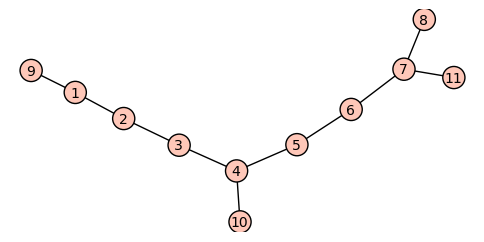
\includegraphics{graphplot.png}
\end{para}
%
\begin{para}
The automorphism group of $D$ has order 2:
\end{para}
%
\begin{sagecode}
\begin{sageinput}
D.automorphism_group().order()
\end{sageinput}
\begin{sageoutput}
2
\end{sageoutput}
\end{sagecode}
%
\begin{para}
and we can determine its orbits:
\end{para}
%
\begin{sagecode}
\begin{sageinput}
D.automorphism_group(return_group=False, orbits=True)
\end{sageinput}
\begin{sageoutput}
[[1], [2], [3], [4], [5], [6], [7], [8, 11], [9], [10]]
\end{sageoutput}
\end{sagecode}
%
\begin{para}
As an alternative to the last command we could try the following, but its
output is misleading!
\end{para}
%
\begin{sagecode}
\begin{sageinput}
D.automorphism_group().orbits()
\end{sageinput}
\begin{sageoutput}
[[1], [2], [3], [4], [5], [6], [7, 10], [8], [9], [11]]
\end{sageoutput}
\end{sagecode}
%
\begin{para}
This is because automorphism groups of graphs do not always exactly match the integer symbols for the permutation group to the names of the vertices.  Here is the translation between vertex names to permutation group symbols, as a Python dictionary.
\end{para}
%
\begin{sagecode}
\begin{sageinput}
D.automorphism_group(return_group=False, translation=True)
\end{sageinput}
\begin{sageoutput}
{1: 11, 2: 1, 3: 2, 4: 3, 5: 4, 6: 5, 7: 6, 8: 7, 9: 8, 10: 9, 11: 10}
\end{sageoutput}
\end{sagecode}
%
\begin{para}
I claim $D$ has a pair of pseudosimilar vertices. In this case we could find them
by inspecting our drawing of $D$, but we work through a general approach.
The idea is to find a canonical label for each of the 11 vertex-deleted subgraphs
of $D$. The sage command
\end{para}
%
\begin{sagecode}
\begin{sageinput}
E = D.canonical_label()
E.edges(labels=False)
\end{sageinput}
\begin{sageoutput}
[(0, 10), (1, 10), (2, 8), (3, 9), (4, 6), 
(4, 10), (5, 7), (5, 8), (6, 9), (7, 9)]
\end{sageoutput}
\end{sagecode}
%
\begin{para}
returns a canonized form of $D$. So graphs $G$ and $H$ are isomorphic if and only if
their canonized forms are equal. For example
\end{para}
%
\begin{sagecode}
\begin{sageinput}
P = graphs.PetersenGraph()
Q = graphs.CompleteGraph(5).line_graph().complement()
Pc = P.canonical_label(); Qc = Q.canonical_label()
P == Q, Pc == Qc
\end{sageinput}
\begin{sageoutput}
(False, True)
\end{sageoutput}
\end{sagecode}
%
\begin{para}
The only problem left is that the return value of \verb|canonical_label()|
is not hashable. We can circumvent this as follows.
\end{para}
%
\begin{para}
The following procedure constructs a hashable canonical label for 
$G\diff i$, given $G$ and $i$.
\end{para}
%
\begin{sagecode}
\begin{sageinput}
def vdi(G, i):
    H = G.copy()
    H.delete_vertex(i)
    return (H.canonical_label().graph6_string(), i)
\end{sageinput}
\end{sagecode}
%
\begin{para}
We can now construct our list of pairs of the form (string, vertex):
\end{para}
%
\begin{sagecode}
\begin{sageinput}
orbs = D.automorphism_group( return_group=False, orbits=True)
orb_reps = [it[0] for it in orbs]
labels = [vdi(D,i) for i in orb_reps]
labels
\end{sageinput}
\begin{sageoutput}
[('I??G?DaDO', 1), ('I_???CpB_', 2), ('I??X??BoO', 3), 
('I???GOPW_', 4), ('I??G_GBw?', 5), ('I??X??BoO', 6), 
('I???Gg_Ag', 7), ('I??OQaGH_', 8), ('I???oH`b?', 9), 
('I?COOIAWO', 10)]
\end{sageoutput}
\end{sagecode}
%
\begin{para}
and on inspecting the output, we see that $D\diff 3\cong D\diff 6$.
\end{para}
%
\begin{para}
As an exercise, construct a graph on 8 vertices with a pair of pseudosimilar
vertices.
\end{para}
%
\begin{para}
Now we describe how to get a list of the sets of vertices such that all
vertices in the same set have the same vertex-deleted subgraphs.
First we need to convert our list of pairs to a dictionary keyed on the 
first term of the pair; the value of a key will be all second terms 
with the same first term. (The keys for a dictionary must be hashable, so this
is why we needed the graph6 strings.)
\end{para}
%
\begin{sagecode}
\begin{sageinput}
def ls_dict( tuples):
    dc = {} 
    for pair in tuples:
        if dc.has_key( pair[0]):
            dc[ pair[0]].append(pair[1])
        else:
            dc[ pair[0]] = [pair[1]]
    return dc
\end{sageinput}
\end{sagecode}
%
\begin{para}
Now if \verb|dc| is a dictionary whose values are lists, we compute a list consisting
of those values whose length is at least $k$:
\end{para}
%
\begin{sagecode}
\begin{sageinput}
def get_families( dc, k):
    families = []
    for str, vxs in dc.iteritems():
        if len(vxs) >= k:
            families.append( vxs)
    return families
\end{sageinput}
\end{sagecode}
%
\begin{para}
We apply this to our list \texttt{labels}:
\end{para}
%
\begin{sagecode}
\begin{sageinput}
get_families( ls_dict( labels), 2)
\end{sageinput}
\begin{sageoutput}
[[3, 6]]
\end{sageoutput}
\end{sagecode}
%
\begin{para}
We see again that 3 and 6 form a pseudosimilar pair of vertices.
\end{para}
%
\begin{para}
For further reading on pseudosimilar vertices, you will have to dig out papers
on the topic.  I suspect that few of these are on the web, since they
predate \LaTeX{}.  Fortunately we still have libraries.  Note that pseudosimilar
sets of size greater than two are possible.
\end{para}
%
\end{sect}
%
\begin{sect}{Circle Graphs}
%
\begin{para}
To construct a \textsl{circle graph} we first choose $n$ pairs of points on a 
circle in the real plane and then join each pair of points by a straight line,
a \textsl{chord}. These chords are the vertices of the circle graph and they
are adjacent if and only if they cross.
\end{para}
%
\begin{para}
In fact we can view our $2n$ points as the vertices on the cycle of length
$2n$, and represent the chords by a perfect matching in the complete graph
on the vertices of the cycle. We call this structure a \textsl{chord diagram}.
This can be viewed as a cubic graph, with a parallel edge wherever the matching
edge is also an edge in the cycle.
Since a matching edge which is parallel to a cycle edge does not cross
another matching edge, it forms an isolated vertex in the circle
graph. For most purposes we can therefore assume that the matching has
no edge in the cycle---it's a subgraph of $\comp{C_{2n}}$.
\end{para}
%
\begin{para}
Chord diagrams arise in knot theory. Suppose we have a knot drawn in the
plane; assume that there are $n$ crossings labelled 1 through $n$. The knot is 
an embedding of a circle and, on walking around this circle we see a sequence
of $2n$ integers. The terms of the sequence are elements of $\{1,\ldots,n\}$,
and each element occurs twice. Such a sequence is known as a 
\textsl{double occurrence word}. We could even encode the actual knot by
assigning $i^+$ to the overpass and $i^-$ to the underpass, but we digress.
Each double occurrence word determines a chord diagram with $n$ chords---
simply write the word on the vertices of $C_{2n}$ in the natural way, and then
join vertices with the same label by an edge.
\end{para}
%
\begin{para}
For the moment at least, we specify a circle graph on $n$ vertices by a 
perfect matching in $K_{2n}$, and thus by a set of $n$ edges.
We need to decide if two edges of the matching cross:
\end{para}
%
\begin{sagecode}
\begin{sageinput}
def cross(e1,e2):
    if e1[1]<e1[0]: e1[0],e1[1] = e1[1],e1[0]
    if e2[1]<e2[0]: e2[0],e2[1] = e2[1],e2[0]
    return (e1[0]<e2[0] and e2[0]<e1[1]<e2[1]) or (e2[0]<e1[0]<e2[1] and e2[1]<e1[1])
\end{sageinput}
\end{sagecode}
%
\begin{para}
With this in hand we can easily construct the circle graph corresponding
to a given matching:
\end{para}
%
\begin{sagecode}
\begin{sageinput}
def circle_grf(pm):
    return Graph([range( len( pm)), lambda i,j: cross(pm[i],pm[j])])
\end{sageinput}
\end{sagecode}
%
\begin{sagecode}
\begin{sageinput}
def chord_dgrm(pm):
    dgrm = graphs.CycleGraph( 2*len(pm))
    dgrm.add_edges( pm)
    return dgrm
\end{sageinput}
\end{sagecode}
%
\begin{sagecode}
\begin{sageinput}
pm = [(0, 8), (1, 4), (2, 9), (3, 6), (5, 7)]
CD = chord_dgrm( pm)
show(CD)  # not tested
\end{sageinput}
\begin{sageoutput}
\end{sageoutput}
\end{sagecode}
%
\begin{para}
We can get the perfect matchings in the complement of $C_{10}$ as follows.
(It's not pretty, but it works.)
\end{para}
%
\begin{sagecode}
\begin{sageinput}
C = graphs.CycleGraph(10)
CC = C.complement().line_graph().complement()
cliques = CC.cliques_maximum()
len(cliques)
\end{sageinput}
\begin{sageoutput}
293
\end{sageoutput}
\end{sagecode}
%
\begin{para}
So there are 293 perfect matchings in the complement of $C_{10}$. It is easy
to create the corresponding circle graphs and then find the number of different possibilities by examining canonical labelings.
\end{para}
%
\begin{sagecode}
\begin{sageinput}
grfs = [circle_grf( pm).canonical_label().graph6_string() for pm in cliques]
uniq = Set(grfs)
uniq
\end{sageinput}
\begin{sageoutput}
{'DBk', 'D]{', 'D`K', 'DK[', 'DBg', 'DB{', 
'D@s', 'D^{', 'D@{', 'D?{', 'Dbk', 'DF{', 
'DIk', 'D@O', 'DJ{', 'DLo', 'DK{', 'D~{', 
'D_K', 'DNw', 'DL{', 'DJk', 'DFw', 'DN{'}
\end{sageoutput}
\end{sagecode}
%
\begin{para}
With just 24 different circle graphs resulting from the 293 matchings, we see this is not a particularly efficient way to generate circle graphs.
\end{para}
%
\begin{para}
We can make use of procedures to convert between perfect matchings and double
occurrence words.
\end{para}
%
\end{sect}
%
\begin{sect}{Line Graphs and Covers}
%
\begin{para}
Let $D$ be the incidence matrix of an orientation of the graph $X$. Then
\[
    DD^T = \De -A,\quad D^TD = 2I +S
\]
where $\De$ is the diagonal matrix of valencies of $X$ and $S$ is a symmetric
matrix with zero diaogonal and off-diagonal entries from $\{0,1,-1\}$.
In other words, $S$ is a \textsl{signed adjacency matrix}. The entries of
$S$ are indexed by $E(X)$, and the $ab$-entry is non-zero if and only if
the edges $a$ and $b$ are adjacent in the line graph $L(X)$ of $X$,
so we have a signed adjacency matrix for $L(X)$.
\end{para}
%
\begin{para}
A signed ajacency matrix $T$ of a graph $Y$ determines a \textsl{two-fold cover} $Z$
of $Y$, as follows. The vertex set of the cover is
\[
    V(Y) \times \{0,1\}
\]
and $(u,i)$ and $(v,j)$ are adjacent if and only if $u\sim v$ and either
\[
    i=j,\quad T_{u,v}=1
\]
or
\[
    i\ne j,\quad T_{u,v}=-1.
\]
It is easy to check that the map that sends $(u,i)$ to $(u,1-i)$ is an automorphism
of $Z$. In matrix terms, we get the adjacency matrix of $Z$ by applying
the following substitutions to the entries of $A(Y)$:
\[
    0\to\pmat{0&0\\0&0},\qquad 1\to\pmat{1&0\\0&1}
        \qquad -1\to\pmat{0&1\\1&0}.
\]
\end{para}
%
\begin{para}
The pairs 
\[
    \{(u,0),(u,1)\}
\]
are called the fibres of the cover, you might verify that these form an equitable
partition of the cover, and that the quotient over the fibres is $Y$. Thus
we see that the characteristic polynomial of the cover is divisible
by the characteristic polynomial of the graph.
\end{para}
%
\begin{para}
%
\begin{lemma}
\begin{statement}
\[
        \phi(Z,t) =\phi(T,t)\phi(Y,t).
\]
\end{statement}    
\begin{proof}
(Outline.) Let $H$ be the matrix
\[
    \frac{1}{\sqrt{2}} \pmat{1&1\\1&-1}
\]
and let $K$ be the block-diagonal matrix formed using $|V(Y)|$ copies of $H$.
If $M$ is a complex matrix, let $|M$ denote the matrix we get by replacing each entry
of $M$ by its absolute value.
Then $K$ is orthogonal and symmetric and $KA(Z)K$ is permutation equivalent to 
\[
    \pmat{S&0\\0&|S|}.
\]
\end{proof}
\end{lemma}
\end{para}
%
\begin{para}
Here $|S|=A(Y)$. We offer another view of this result.
If $A$ and $B$ are symmetric $01$-matrices such that $A\circ B=0$,
then $A-B$ is a signed adjacency matrix and
\[
    \pmat{A&B\\B&A}
\]
is the adjacency matrix of the corresponding cover.
We can now use the following:
\[
    \frac12\pmat{I&I\\I&-I}\pmat{A&B\\B&A}\pmat{I&I\\I&-I}
        =\pmat{A+B&0\\0&A-B}.
\]
\end{para}
%
\begin{para}
This leads us to an easy construction of the adjacency matrix of the cover.
\end{para}
%
\begin{sagecode}
\begin{sageinput}
def lgcvr( X):
    D = X.incidence_matrix()
    IDM = identity_matrix( X.num_edges())
    M = D.transpose()*D -2*IDM
    MM = M.elementwise_product(M)
    A = (1/2)*(M+MM)
    B = (1/2)*(M-MM)
    return block_matrix(2, 2, [A,B,B,A])
\end{sageinput}
\end{sagecode}
%
\begin{para}
Now we turn to our line graphs. The cover can be constructed as follows.
Choose one arc $(u,v)$ for each edge $\{u,v\}$ of $X$. (This defines an orientation
of the graph.) Our matrix $S$ is a signing of $A(L(X))$---its rows and columns
are indexed by our chosen arcs, and the entry corresponding to a pair
of distinct overlapping arcs is 1 if they have the same head or tail,
and $-1$ otherwise. Rather than represent the vertices of the cover by
pairs $((u,v),i)$, we proceed thus: if $(u,v)$ is one of our chosen
arcs then we use $(u,v)$ to denote $((u,v),0)$ and $(v,u)$ for $((u,v),1)$.
The following procedure implements this.
\end{para}
%
\begin{sagecode}
\begin{sageinput}
def dbl_lng( X):
    V = X.vertices()
    E = X.edges( labels=False)
    arcs = [(i,j) for i in V for j in V\
        if ((i,j) in E or (j,i) in E)]
    return  Graph( [arcs, lambda a,b: a != b and (a[0]==b[0] or a[1]==b[1])])
\end{sageinput}
\end{sagecode}
%
\begin{para}
We test that our two constructions agree on the Petersen graph, and see
that cover is isomorphic to the line graph of the direct product of
the Petersen graph with $K_2$. (This product is itself a cover of the Petersen
graph.)
\end{para}
%
\begin{sagecode}
\begin{sageinput}
P = graphs.PetersenGraph()
Q1 = Graph( lgcvr( P))
Q2 = dbl_lng( P)
Q1.is_isomorphic( Q2)
\end{sageinput}
\begin{sageoutput}
True
\end{sageoutput}
\end{sagecode}
%
\begin{sagecode}
\begin{sageinput}
K2 = graphs.CompleteGraph(2)
LP2 = (P.tensor_product(K2)).line_graph()
LP2.is_isomorphic( Q1)
\end{sageinput}
\begin{sageoutput}
True
\end{sageoutput}
\end{sagecode}
%
\end{sect}
%
\end{chap}
%!TEX root = Practice.tex

\chapter{Cayley Graphs}

\section{Cayley Graphs}

If $G$ is a group and $C\sbs G$ (i.e., a list of some elements of $G$), then the 
command produces the Cayley graph $X(G,C)$:
\begin{verbatim}
    G.cayley_graph( generators = C)
\end{verbatim}
The output is a directed graph, even if $C$ is inverse-closed; in the latter
case we can convert $G$ to a graph by
\begin{verbatim}
    H = G.to_undirected()
\end{verbatim}
Note that $C$ is not required to generate $G$. There are a number of keywords
to this command (for example, \texttt{side} and \texttt{simple}) but I cannot
follow their documentation and so I do not know what they do.

Note that the \texttt{Graph()} command makes it easy to construct Cayley
graphs ourselves. For example, a \textsl{cubelike graph} is a Cayley
graph for $GF(2)^d$. We can construct them using \texttt{Graph()}.
\begin{verbatim}
def cubelike(d, vector_list):
    VS = VectorSpace(GF(2),d)
    vxs = range{2^d}
    return Graph([vxs, lambda i,j: VS[i]-VS[j] in vector_list])
\end{verbatim}
Here \verb|vector_list| is a list of 01-vectors of length $d$
For a general group, we can use the following.
\begin{verbatim}
    CG = Graph( [ G.list(), lambda g, h: h*g^(-1) in C])
\end{verbatim}
This will produce an incorrect result if $C$ is not inverse-closed.

Sage provides access to GAP, and hence access to any group that is
in GAP or can be constructed in GAP.  Be warned that the documentation
for GAP probably outweighs that for sage.


\section{The Higman-Sims Graph}

We construct the famous Higman-Sims graph as a Cayley graph for a permutation
group. Our code is based on an interesting paper by Jorgensen and Klin
from the Electronic Journal of Combinatorics
(\url{http://www.combinatorics.org/Volume_10/PDF/v10i1r17.pdf}).
They provide constructions for a number of srg's on 100 vertices.

First we form a permutation group.
\begin{sageblock}
    H1 = PermutationGroup([[(1,2,3,4,5)],[(6,7,8,9,10)],\
      [(2,3,5,4)]])
\end{sageblock}
The argument to \texttt{PermutationGroup()} is a list where each item in the
list is a list of cycles. Using \verb|H1.order()| shows that \verb|H1| has 
order 100 while \verb|H1.gens()| provides a list of generators---naturally they 
are the three elements we used, but in a different order.
The command \verb|H1.cayley_graph()| will return a directed Cayley graph using
the elements of \verb|H.gens()| as the connection set.

Obviously, to get the Higman-Sims graph we need a special connection set.
For this we make use of the following set of 22 triples:
\begin{sageblock}
ds = [(1,0,0), (4,0,0), (0,1,1), (0,4,1), (2,0,1), (4,2,1),\
  (4,3,1), (0,1,2), (0,4,2), (1,2,2), (1,3,2), (2,0,2),\
  (3,1,2), (3,2,2), (3,3,2), (3,4,2), (4,0,2), (0,1,3),\
  (0,4,3), (1,0,3), (2,2,3), (2,3,3)]
\end{sageblock}
We set
\begin{sageblock}
    y,z,x = H1.gens()
\end{sageblock}
and then create a connection set
\begin{sageblock}
    C = [ x^it[0]*y^it[1]*z^it[2] for it in ds]
\end{sageblock}
Here $x$, $y$ and $z$ are our original generators and $C$ is a subset
of $G$ consisting of elements of the form $x^iy^jz^k$. So they are
specified by triples $(i,j,k)$ and \verb|ds| is indeed a set of triples.
We could perform a partial check on our work by testing if $C$ is inverse-closed.
The graph we want is
\begin{sageblock}
    G = H1.cayley_graph( generators=C)
\end{sageblock}

How can we confirm that this is the Higman-Sims graph?  Well, it is connected,
regular, and has exactly three eigenvalues:

\begin{sageexample}
    sage: G.is_connected()
    sage: G.is_regular()
    sage: G.am().fcp()
\end{sageexample}

Since the Higman-Sims graph is determined by its eigenvalues, we have it.
We could use \verb|G.girth()| to see that $G$ is triangle-free.
We used \verb|G.am().fcp()| to get the factored characteristic polynomial
of $G$, because it's shorter than \verb|G.characteristic_polynomial().factor()|
even with tab completion. Also, for a graph on any significant number of vertices
there is very little to be gained by looking at the coefficients of its
characteristic polynomial---they are far too large!

We can see that $G$ is vertex transitive by invoking \verb|G.is_transitive()|.
To verify that $G$ is arc-transitive, we prove more by showing
that the stabilizer of a vertex has exactly three orbits on vertices.
We set things up with
\begin{sageblock}
    G.relabel()
    part = [[0], [1..99]]
    orbs = G.automorphism_group( return_group=False,\
      partition=part, orbits=True)
\end{sageblock}
Some explanations are in order. As created the vertices of $G$ are permutations,
after \verb|G.relabel()| they are the integers in $[0..99]$. Now
\verb|dist_part| is the distance partition of $G$ relative to the vertex $0$
and \verb|orbs| is the list of orbits of the subgroup of automorphisms of $G$
that fix each cell of the partition \texttt{part}. From
\begin{sageexample}
    sage: len(orbs)
\end{sageexample}
we infer that the vertex stabiliser has three orbits, which must be 0,
the neighbors of 0 and the vertices at distance two from 0. We conclude
that $\aut G$ is a rank-three permutation group. Its order?
\begin{sageexample}
    sage: G.automorphism_group(return_group=False,order=True)
\end{sageexample}

The Higman-Sims graphs contains many triangle-free srg's as subgraphs.
For example, the subgraphs obtained by deleting a vertex and its neighbors
or by deleting two adjacent vertices and its neighbors. Its vertices
can be partitioned into two copies of the Hoffman-Singleton graph,
but that's another story.

\section{The 600-Cell}

It's a wikifact that if $f:=(1+\sqrt{5})/2$, then the vertices of a 600-cell 
centered at the origin of 4-space with edges of length $1/f$ 
can be given as follows: 
\begin{enumerate}
    \item
    16 vertices of the form
    \[
        \frac12(\pm1,\pm1,\pm1,\pm1),
    \]
    \item
    8 vertices obtained all permutations of the coordinates of
    \[
        (\pm1,0,0,0)
    \]
    \item
    96 vertices obtained by taking all even permutations of
    \[
        \frac12\left(\pm1,\pm f,\pm f^{-1},0\right).
    \]
\end{enumerate}  
The first step is produce a $120\times4$ matrix $U$ with these vectors
its rows. The game is to do this without using a for-loop.
We set up our background
\begin{sageblock}
    x = QQ['x'].0
    K.<f> = NumberField(x^2-x-1)
    RR4 = VectorSpace(K,4) 
    H.<i,j,k> = QuaternionAlgebra(K,-1,-1)
\end{sageblock}
So we work with quaternions over $\rats(f)$, where $f$ is a zero of $f^2-f-1$.
Due t an unfortunate feature of python, we must remember now \textbf{never}
to use $i$ or $j$ or $k$ as an index in a list comprehension---after
executing
\begin{verbatim}
    [i^2 for i in [1..5]]
\end{verbatim}
the value of $i$ is now 5.

Now we create $U$. 
\begin{sageblock}    
    CP3 = CartesianProduct([-1,1],[-1,1],[-1,1],[0])
    CP4 = CartesianProduct([-1,1],[-1,1],[-1,1],[-1,1])
    fv1 = RR4([1/2,f/2,(f-1)/2,0])
    fv2 = RR4([(f-1)/2,1/2,f/2,0])
    fv3 = RR4([f/2,(f-1)/2,1/2,0])
    xx= [fv1.pairwise_product(RR4(sign_v))\
      for sign_v in CP3]\
     +[fv2.pairwise_product(RR4(sign_v))\
      for sign_v in CP3]\
     +[fv3.pairwise_product(RR4(sign_v))\
      for sign_v in CP3]
    mm = Matrix(xx)
    mma = mm.matrix_from_columns([1,0,3,2])
    mmb = mm.matrix_from_columns([2,3,0,1])
    mmc = mm.matrix_from_columns([3,2,1,0])
    MM = block_matrix([mm,mma,mmb,mmc], nrows=4)
    ww = RR4([1/2,1/2,1/2,1/2])
    xxd =\ 
      [ww.pairwise_product(RR4(sign_v))\
      for sign_v in CP4]+[RR4([1,0,0,0]),\  
      RR4([-1,0,0,0]),RR4([0,1,0,0]),RR4([0,-1,0,0]),\ 
      RR4([0,0,1,0]), RR4([0,0,-1,0]),RR4([0,0,0,1]),\
      RR4([0,0,0,-1])]
    U = MM.stack(Matrix(xxd))
\end{sageblock}
The best we can say for the above code is that it works. Interestingly
enough, the columns of $U$ are orthogonal $U^TU =30I$.

Two vectors are adjacent in the 1-skeleton if their inner product is $1/f$.
\begin{sageblock}
    DC = Graph([[1..120],\
     lambda i,j: U[i-1].inner_product(U[j-1]) == 1/2*f])
\end{sageblock}

\begin{sageexample}
sage: DC.is_regular()
sage: DC.is_vertex_transitive()
sage: DC.degree()[0]
sage: DC.diameter()
\end{sageexample}

We compute the orbits of the vertex stabilizer of $\aut{DC}$.
\begin{sageexample}
sage: DCgrp = DC.automorphism_group( partition = [[1],[2..120]])
sage: map( len, DCgrp.orbits())
\end{sageexample}

We convert the rows of $U$ to quaternions.
\begin{sageblock}
qu = [uu[0]+uu[1]*i+uu[2]*j +uu[3]*k for uu in U.rows()]
\end{sageblock}
The reduced trace of a quaternion $q$ is $q+q^*$, in other words it is
twice its real part. The multiplicative order of a quaternion is determined
by its real trace. We compute the partition of $qu$ by reduced trace
\begin{sageblock}
tuples = [(qq.reduced_trace(),qq) for qq in qu]
dc = ls_dict( tuples)
\end{sageblock}

\begin{sageexample}
sage: [(kit, len(dc[kit])) for kit in dc.keys()]
\end{sageexample}
Comparing the number of quaternions with given reduced trace with the
sizes of the orbits of the vertex stabilizer, suggests that the two partitions
are equal. You should verify this. You should also verify that the
multiplicative order of an element of \verb|qu|. (Use \verb|qq.order()|.)
is determined by its reduced trace. In particular the quaternions
with reduced trace $f$ or$1-f$ have order 10. The quaternions in
\verb|qu| form a multiplicative group isomorphic to $SL(2,5)$.
You can access this group in sage by
\begin{verbatim}
    T = SL(2,5).
\end{verbatim}

The 600-cell is a Cayley graph for this group with connection
set consisting of a conjugacy class of elements of order 10.
There are two such conjugacy classes, one formed by the elements
with reduced trace $f$ and the other consisting of the elements of reduced
trace $1-f$. We show now that the Cayley graph with respect to the first of these
conjugacy classes is isomorphic to $DC$, you should verify that the second is.
\begin{sageblock}
    rtf = [it for it in qu if it.reduced_trace() == f]
    conn = Set([ it^(-1)*rtf[0]*it for it in qu]).list()
    CG = Graph( [qu, lambda q1, q2: q2*q1^(-1) in conn])
\end{sageblock}
and now
\begin{sageexample}
sage: CG.is_isomorphic( DC)
\end{sageexample}

The quaternion
\[
    th = (-1/2) + 1/2*i + 1/2*j + 1/2*k
\]
has order three and its orbits on $DC$ are cocliques. The quotient
over its orbits is graph on 40 vertices which, like \verb|DC|, is locally
an icosahedron. We confirm the first claim:

\begin{sageexample}
sage: nbhd = DC.subgraph( vertices=DC[1])
sage: nbhd.is_isomorphic( graphs.IcosahedralGraph())
\end{sageexample}


\section{Cubelike Graphs}

A cubelike graph is a Cayley graph for $\ints_2^d$. The connection
set of such a graph can be encoded by a $d\times m$ matrix with distinct
columns. If $M$ is such a matrix then we can get a list of its columns by
\begin{verbatim}
    cols = M.columns()
\end{verbatim}
and we can recover $M$ by
\begin{verbatim}
    M = Matrix(cols).transpose()
\end{verbatim}
The natural choice for the vertices of a cubelike graph are the elements of
\begin{verbatim}
    V = VectorSpace( GF(2)), d)
\end{verbatim}
but these are not hashable. We can make a vector \verb|v| hashable by
\begin{verbatim}
    v.set_immutable()
\end{verbatim}
and use vectors as vertices, or work as follows.
\begin{verbatim}
    G = Graph( [[0..len(vls)-1],\
     lambda i,j: vls[i]-vls[j] in V.list()])
\end{verbatim}

\begin{verbatim}
    P = graphs.PetersenGraph()
    D = P.incidence_matrix()
    B = D.change_ring( GF(2)) # convert to a matrix over GF(2)
    B0 = B.submatrix( nrows=B.nrows()-1) # delete last row
\end{verbatim}

For humans it can be convenient to encode binary vectors of length $d$ as 
integers between 0 and $2^{d-1}$. With $G$ as just defined, its connection
set will be the correct set of integers.

\begin{verbatim}
def cubelike(vecls):
    d = len(vecls[0])
    VS = VectorSpace(GF(2),d)
    return Graph([[0..(2^d-1)],\
     lambda i,j: VS[i]-VS[j] in vecls])
\end{verbatim}
\begin{chap}{Distance-Regular Graphs}{drgs}
%
\begin{sect}{Distance Regularity}
%
\begin{para}
First some code to allow us to test if a graph is distance regular.
The main use of this is to provide a test that some graph we have constructed is
distance regular.
\end{para}
%
\begin{sagecode}
\begin{sageinput}
def distance_partition( X, vxi):
    xvs = X.vertices()
    E = dict()
    for vxj in xvs:
        dj = X.distance(vxi, vxj)
        E.setdefault(dj,[]).append(vxj)
    return E.values()    
\end{sageinput}
\end{sagecode}
%    
\begin{para}
If $X$ is distance-regular, then the distance partition is equitable
and the quotient matrix with respect to this partition is the same for all
vertices. 
\end{para}
%
\begin{para}
We use the Kneser graphs as a test case, though we must relabel the vertices to convert them from sets to integers.
\end{para}
%
\begin{sagecode}
\begin{sageinput}
X = graphs.KneserGraph(7, 3)
X.relabel()
dp = distance_partition( X, X.vertices()[0])
X.is_equitable( dp, quotient_matrix=True) 
\end{sageinput}
\begin{sageoutput}
[0 4 0 0]                               
[1 0 3 0]                               
[0 1 0 3]                               
[0 0 2 2]
\end{sageoutput}
\end{sagecode}
%
\begin{para}
If the partition is not equitable, the response would be a simple
\verb|False|.
\end{para}
%
\begin{para}
Many distance-regular graphs are distance-transitive. We can test for this
by verifying that our graph is vertex transitive and the number of
orbits of the stabilizer of a vertex is the diameter plus one.
\end{para}
%
\begin{sagecode}
\begin{sageinput}
orbs = X.automorphism_group( return_group=0, orbits=1)
len(orbs) == 1 
\end{sageinput}
\begin{sageoutput}
True
\end{sageoutput}
\end{sagecode}
%
\begin{sagecode}
\begin{sageinput}
pn = [ [X.vertices()[0]], X.vertices()[1:]]
grp = X.automorphism_group( partition=pn)
len( grp.orbits()) == X.diameter() + 1
\end{sageinput}
\begin{sageoutput}
True
\end{sageoutput}
\end{sagecode}
%
\begin{para}
The Kneser graph has a perfect 1-code---a set of seven vertices pairwise at distance
three. If we delete the vertices in a perfect 1-code, the resulting graph
is the Coxeter graph which is a distance-regular cubic graph.
It is not too hard to see that a perfect 1-code will be a coclique of size seven
that is maximal under inclusion. So we can find one and construct the
Coxeter graph as follows.
\end{para}
%
\begin{sagecode}
\begin{sageinput}
colqs = X.complement().cliques_maximal()
colqs7 = filter( lambda it: len(it)==7, colqs)
Y = X.copy()
Y.delete_vertices( colqs7[0])
\end{sageinput}
\end{sagecode}
%
\begin{para}
We confirm that $Y$ has girth seven, an increase of one from the girth of $X$.  You might verify that $Y$ is distance-transitive.
\end{para}
%
\begin{sagecode}
\begin{sageinput}
X.girth(), Y.girth()
\end{sageinput}
\begin{sageoutput}
(6, 7)
\end{sageoutput}
\end{sagecode}
%
\end{sect}
%
\begin{sect}{Generalized Quadrangles}
%
\begin{para}
A \textsl{generalized quadrangle} is an incidence structure of points
and lines such that
\end{para}
%
\begin{enumerate}
    \begin{listitem}
    Any two points lie on at most one line.
    \end{listitem}
    \begin{listitem}
    If the point $x$ is off the line $\ell$, then there is a unique
    point on $\ell$ collinear with $x$.
    \end{listitem}
\end{enumerate}
%
\begin{para}
These axioms are self-dual, and therefore the incidence structure
dual to a $GQ$ is again a $GQ$.
\end{para}
%
\begin{para}
The smallest interesting example has as points the 15 edges of $K_6$ and
as lines the 15 1-factors of $K_6$; each edge is incident with the three
1-factors that contain it. A $GQ$ is \textsl{thick} if each point is on at least 
three lines and each line contains at least three points. If a $GQ$ is thick then
it is point and line regular, this means there are integers $s$ and $t$ such that
each point lies on exactly $t+1$ lines and each line contains exactly $s+1$
points. Our example above is a $GQ(2,2)$, traditionally denoted by $W(2)$.
\end{para}
%
\begin{para}
Associated to an incidence structure we have a point graph, a line graph
and an incidence graph.  For $W(2)$ the point and line graphs are isomorphic
to $L(K_6)$ (which is very easy to check); the incidence graph is
a bipartite cubic graph on 30 vertices with diameter four and girth eight.
It is known as \textsl{Tutte's 8-cage}. For a thick $GQ$, both the point
and line graphs are strongly regular.
\end{para}
%
\begin{para}
We describe how to construct a family of $GQ$'s denoted by $W(q)$, where
$q$ is a primes power. We will accompany the description with the
code for $W(3)$.
\end{para}
%
\begin{para}
Let $V$ be the vector space of dimension four over $GF(q)$. Its 1-dimensional
subspaces will be the points of our generalized quadrangle. To define
the lines we want a non-degenerate alternating form on $V$; this is
given by an invertible matrix $S$ with diagonal entries zero such that $S+S^T=0$.
(So if $q$ is odd, then $S$ is skew symmetric; if $q$ is even it's symmetric
with zero diagonal.) A subspace $U$ of $V$ is \textsl{isotropic}
if
\[
    u^THv = 0
\]
for all $u$, $v$ in $U$. All 1-dimensional subspaces of $V$ are isotropic and the
lines of $W(q)$ will be the 2-dimensional isotropic subspaces.
\end{para}
%
\begin{para}
Time for some actual work. We define our form:
\end{para}
%
\begin{sagecode}
\begin{sageinput}
def beta(u,v):
    return u[0]*v[2]+u[1]*v[3] -u[2]*v[0] -u[3]*v[1]
\end{sageinput}
\end{sagecode}
%
\begin{para}
and create our points and lines:
\end{para}
%
\begin{sagecode}
\begin{sageinput}
V = VectorSpace( GF(3), 4)
pnts = [u[1] for u in V.subspaces(1)]
lines = [sub for sub in V.subspaces(2)\
    if beta(sub.matrix()[0],sub.matrix()[1])==0]
\end{sageinput}
\end{sagecode}
%
\begin{para}
Two points $u$ and $v$ are collinear if $\beta(u,v)=0$. Two lines $L$ and $M$ 
are incident if
\end{para}
%
\begin{sagecode}
\begin{sageinput}
(L != M) and (L.intersection(M) != V.zero_subspace()) # not tested
\end{sageinput}
\end{sagecode}
%
\begin{para}
or if they are not equal and
\end{para}
%
\begin{sagecode}
\begin{sageinput}
det( L.matrix().stack(M.matrix)) == 0 # not tested
\end{sageinput}
\end{sagecode}
%
\begin{para}
Elements of our vector space $V$ are "mutable", so not hashable, 
and therefore cannot be used as vertices of a graph. This is easily circumvented:
\end{para}
%
\begin{sagecode}
\begin{sageinput}
adj = lambda i,j: beta(pnts[i],pnts[j])==0
W3 = Graph([range(len(pnts)),adj], loops=False)
\end{sageinput}
\end{sagecode}
%
\begin{para}
We can check that $W3$ is connected and regular, and that it has exactly three
eigenvalues (obvious in the factored characteristic polynomial):
\end{para}
%
\begin{sagecode}
\begin{sageinput}
W3.is_connected(), W3.is_regular(), W3.am().fcp()
\end{sageinput}
\begin{sageoutput}
(True, True, (x - 12) * (x + 4)^15 * (x - 2)^24)
\end{sageoutput}
\end{sagecode}
%
\begin{para}
The lines of the $GQ$ correspond to the cliques of maximal size, which we
can find by
\end{para}
%
\begin{sagecode}
\begin{sageinput}
cliques = W3.cliques_maximum()
\end{sageinput}
\end{sagecode}
%
\begin{para}
We get the point graph of the dual $GQ$ by
\end{para}
%
\begin{sagecode}
\begin{sageinput}
adj = lambda i,j: i != j and det( lines[i].matrix().stack(lines[j].matrix())) == 0
W3d = Graph( [range(len(lines)), adj])
\end{sageinput}
\end{sagecode}
%
\begin{para}
As expected $W3d$ is not isomorphic to $W3$, but it is strongly regular with
the same parameters.
\end{para}
%
\begin{sagecode}
\begin{sageinput}
W3.is_isomorphic(W3d)
\end{sageinput}
\begin{sageoutput}
False
\end{sageoutput}
\end{sagecode}
%
\begin{sagecode}
\begin{sageinput}
dp = distance_partition( W3, W3.vertices()[0])
W3.is_equitable( dp, quotient_matrix=True) 
\end{sageinput}
\begin{sageoutput}
[ 0 12  0]
[ 1  2  9]
[ 0  4  8]
\end{sageoutput}
\end{sagecode}
%
\begin{sagecode}
\begin{sageinput}
dp = distance_partition( W3d, W3d.vertices()[0])
W3d.is_equitable( dp, quotient_matrix=True) 
\end{sageinput}
\begin{sageoutput}
[ 0 12  0]
[ 1  2  9]
[ 0  4  8]
\end{sageoutput}
\end{sagecode}
%
\end{sect}
%
\begin{sect}{The McLaughlin Graph}
%
\begin{para}
A partition $(S,\comp{S})$ of $V(G)$ determines a bipartite subgraph of $G$;
if we replace this subgraph by its bipartite complement, we say that the
resulting graph is got by \textsl{switching} on $S$ (or on $\comp{S}$).
If $S$ is the neighborhood of a vertex $u$ in $G$, then after switching
on $S$ the vertex $u$ is isolated.
\end{para}
%
\begin{sagecode}
\begin{sageinput}
def switch(G,sub):
    H = G.copy()
    rest = Set(H.vertices()).difference(Set(sub))
    for u in sub:
        for v in rest:
            if H.has_edge(u,v): H.delete_edge(u,v)
            else: H.add_edge(u,v)
    return H   
\end{sageinput}
\end{sagecode}
%
\begin{para}
We construct a graph on the blocks of the $4$-$(23,7,1)$ design
formed by the words of weight seven in the binary Golay code of length 23.
(This graph is strongly regular.)
We then add 23 vertices $\{0,\ldots,23\}$ corresponding to the 23 coordinate 
positions of a code word, and join the $i$-th new vertex to the blocks
that do not contain it. The resulting graph is not regular but if we switch on
one of the new vertices and then delete it we get the McLaughlin graph
on 275 vertices, which is strongly regular.
\end{para}
%
\begin{sagecode}
\begin{sageinput}
C = ExtendedBinaryGolayCode()
D = C.punctured([0])
words = [ tuple(it.support()) for it in D if hamming_weight(it)==7]
MG = Graph( [words, lambda a,b: len(Set(a).intersection(Set(b)))==1])
MM = MG.copy()
MM.add_vertices([0..22])
edges = [ (i,a) for i in [0..22] for a in words if i not in a]
MM.add_edges( edges)
McL = switch( MM, MM[0])
McL.delete_vertex(0)
\end{sageinput}
\end{sagecode}
%
\begin{para}
It's strongly regular, with a big automorphism group:
\end{para}
%
\begin{sagecode}
\begin{sageinput}
grp_order = McL.automorphism_group(return_group=0,order=1)
McL.is_connected(), McL.is_regular(), McL.am().fcp(), grp_order
\end{sageinput}
\begin{sageoutput}
(True, True, (x - 112) * (x + 28)^22 * (x - 2)^252, 1796256000)
\end{sageoutput}
\end{sagecode}
%
\begin{para}
The McLaughlin graph gives rise to a regular two-graph. For details on regular
two-graphs, see any recent book on algebraic graph theory. 
\end{para}
%
\begin{sagecode}
\begin{sageinput}
G = McL.copy()
G.relabel()
G.add_vertex()
A = G.am()
n = G.num_verts()
J = Matrix(n,n,n^2*[1])
B = J -1 -A
C = block_matrix( 2, 2, [A,B,B,A])
SMcL = Graph( C)
grp = SMcL.automorphism_group()
grp.order(), SMcL.am().fcp()
\end{sageinput}
\begin{sageoutput}
(991533312000, (x - 275) * (x + 55)^23 * (x - 5)^253 * (x + 1)^275)
\end{sageoutput}
\end{sagecode}
%
\begin{para}
and now
\end{para}
%
\begin{sagecode}
\begin{sageinput}
grp.composition_series()[1].is_simple()
\end{sageinput}
\begin{sageoutput}
True
\end{sageoutput}
\end{sagecode}
%
\begin{para}
The group is one of Conway's simple groups.  [* Too big by a factor of two!  Does the graph need adjustment or does the simple group just come as an index 2 subgroup of the automorphism group? *]
\end{para}
%
\end{sect}
%
\begin{sect}{Drackns: Generating Parameter Sets}
%
\begin{para}
We are interested in distance-regular antipodal covers of $K_n$.
First we explain `cover'. We construct a \textsl{cover} of
index $r$ of a graph $X$ (or an \textsl{$r$-fold cover})
as follows. Choose a function $f$ from the arcs (ordered pairs of adjacent
vertices of $X$) to the symmetric group $\sym r$, such that
\[
    F((v,u)) =f((u,v))^{-1}
\]
The vertex set of the cover $X^f$ is 
\[
    V(X)\times \{1,\ldots,r\}
\]
and $(u,i)\sim (v,j)$ if $j = i^{f(u,v)}$. Less formally, we replace each
vertex of $V(X)$ by a coclique of size $r$, and cocliques corresponding
to adjacent vertices are joined by a matching of size $r$. The $r$-cocliques
are called the \textsl{fibers} of the cover.
\end{para}
%
\begin{para}
A cover $X^f$ is \textsl{antipodal} if its diameter is $d$ and two vertices
are in the same fiber if and only they are at distance $d$. The 3-cube is an antipodal
cover of $K_4$ with index two and diameter three. The line graph of the Petersen
graph is an antipodal cover of $K_5$ with index and diameter three.
\end{para}
%
\begin{para}
Here we are concerned with distance-regular antipodal covers of complete graphs $K_n$.
Such covers must have diameter three. There are four obvious parameters $(n,r,a_1,c_2)$,
although these are not independent, in fact counting edges joining neighbors
of $u$ to vertices at distance two from $u$, we get
\[
    n(n-2-a_2) = n(r-1)c_2
\]
whence
\begin{equation}
\label{eq:n1rc2}
    n-1-rc_2 = a_1-c_2.
\end{equation}
The difference $a_1-c_2$ occurs frequently, and we denote it by $\de$.
It is not too hard to show that an antipodal
cover of $K_n$ is distance regular if its diameter is three and any two 
distinct non-adjacent vertices have $c_2$ common neighbors.
\end{para}
%
\begin{para}
Our basic problem is to determine the parameter triples $(n,r,c_2)$
for which a cover exists. This is an impossible problem, so we settle
for generating parameter sets for which there is a good chance that a
cover exists. Here our first design question surfaces: do we want to order
our parameters by $n$ and then $r$ (lexicographically), or by $nr$ then $r$
(for example). We arbitrarily select the first approach.
\end{para}
%
\begin{para}
As a first step we aim to generate a list of quadruples $(n,r,a_1,c_2)$.
Now we know that
\begin{equation}
\label{eq:rbnd}
    2\le r\le n-1.
\end{equation}
What about $c_2$. The neighborhood of a vertex induces a regular graph
on $n-1$ vertices with valency $a_1$, whence $na_1$ must be even.
From (\ref{eq:n1rc2}) we have 
\[
    n-1-a_1 = (r-1)c_2,
\]
from which we infer that if $n$ is odd and $r$ is even, then $c_2$ must be
even. We also have
\begin{equation}
\label{c2bnd}
    1\le c_2 \le \left\lfloor\frac{n-1}{r-1}\right\rfloor
\end{equation}
\end{para}
%
\begin{sagecode}
\begin{sageinput}
    def nrc( n):
        lim = (n-1)/(r-1)
        return [(n,r,c) for r in [2..n-1]\ 
         for c in [1..lim] and n*(r-1)*c % 2 == 0]
    def get_a( n, r, c):
        return n, r, n-1-(r-1)*c, c
\end{sageinput}
\end{sagecode}
%
\begin{para}
So we will generate a sequence of 4-tuples, and filter out the ones
that obviously do not work. The most useful condition rests on the formulas
for the multiplicities of the eigenvalues. As a distance-regular graph
with diameter three, a drackn has exactly four distinct eigenvalues
\[
    n > \th > -1 > \tau
\]
where $n$ is simple, $-1$ has multiplicity $n-1$ and $-\th\tau=n-1$.
The eigenvalues $\th$ and $\tau$ are the zeros of
\[
    t^2 -\de t - (n-1).
\]
It is their multiplicities that interest us. With an obvious notation we have
\begin{align*}
    rn &= 1 + (n-1) +m_\th+m_\tau\\
    0  &= (n-1) +(n-1)(-1) +m_\th\th+m_\tau\tau
\end{align*}
and therefore
\begin{equation}
\label{eq:mult}
    m_\th = \frac{(r-1)n(-\tau)}{\th -\tau}.
\end{equation}
\end{para}
%
\begin{para}
Two cases arise. First, if $\th$ and $\tau$ are not integers, then
\[
    \th=\sqrt{n-1},\quad \tau=-\sqrt{n-1}
\]
and their multiplicities are equal to $n(r-1)/2$. Otherwise they are integers
and consequently the discriminant
\begin{equation}
\label{eq:discr}
    (\th-\tau)^2 = \de^2+4(n-1) = (a_1-c_2)^2+4(n-1)
\end{equation}
must be a perfect square. (Note that $\de=n-1-rc_2$.) If this is a perfect square
we can determine $\th$ and $\tau$, and then check that our formula for $m_th$
is an integer.
\end{para}
%
\begin{sagecode}
\begin{sageinput}
def mult_chk( n, r, a, c):
    disc = (a-c)^2+4*(n-1)
    if is_square(disc):
        sqroot = sqrt( disc)
        theta = (a-c+sqroot)/2
        tau = (a-c-sqroot)/2
        mth = n*(r-1)*theta/sqroot
        mtau = n*(r-1)-mth
        return (theta, tau, mth, mtau)
    else:
        return False
\end{sageinput}
\end{sagecode}
%
\begin{para}
How do we generate 4-tuples? The simplest approach is to use \verb|CartesianProduct|,
but a more efficient strategy is to use generators.
\end{para}
%
\begin{para}
Now we can generate a selected family of 4-tuples. There are other conditions
that must hold, we write a predicate for each of these and then write
a function that takes a 4-tuple and applies each term in a list of
predicates. Note that, when a parameter set is eliminated we need to know
at least one of the predicates that it fails.
\end{para}
%
\begin{para}
There is a very strong case to be made that a better parameterization is available.
The idea is to search on triples
\[
    (-\tau,\theta, r)
\]
Our approach above throws out most triples because $(a_1-c_2)^2+4(n-1)$ is not
a perfect square. Our alternative approach only produces triples where
this condition is satisfied. We need to treat separately the case where
$m_\th=m_\tau$, (equivalently $\de=0$) but this makes sense combinatorially. 
If we want the parameters for covers of $K_n$ with index $r$, then we filter
through the pairs $(-\tau, \theta)$ where $\theta$ runs over the elements
of \verb|divisors(n-1)| such that the Krein bound holds.
\end{para}
%
\end{sect}
%
\end{chap}
\begin{chap}{Polynomials and Power Series}
%
\begin{sect}{Forbidden Words}
%
\begin{para}
Let $\al$ denote a binary string, and let $L$ denote
the set of binary of binary strings that do not contain $\al$ as a substring. 
How many strings are there in $L$ with length $n$?
\end{para}
%
\begin{para}
Let $M$ denote the binary
strings that contain exactly one copy of $\al$, as a suffix. 
If $\eps$ denotes the empty string, then
\begin{equation}
    \label{eq:eL01}
    \eps+L(0+1) = L+M.
\end{equation}
Also $L\al$ clearly contains $M$ as a subset, but for example if $\al=111$,
then
\[
    L\al =M+M1+M11.
\]
We develop a precise description of $L\al$. Let $\al\backslash\be$ denote the 
set of suffixes $\be_1$ such that
$\be_0\be_1=\be$ and $\be_0$ is a suffix of $\al$. For example if
\[
    \al =100110,\quad \be=1011,
\]
then
\[
    \al\backslash\be = \{11\},\quad \al\backslash\al = \{\eps,0110\}
\]
%
\begin{lemma}
    \[
        L\al = M\al\backslash\al.
    \]
\end{lemma}
\end{para}
%
\begin{para}
Note that $\al\backslash\al$ is a finite language, i.e., a finite set of strings.
\end{para}
%
\begin{para}
If $N$ is a set of binary strings, let $N(t)$ denote its generating series.
This is what we get when we substitute $t$ for $0$ and $1$, a string of length
$\ell$ maps to $t^\ell$ and the language maps to its generating series.
Now \eqref{eq:eL01} yields
\[
    1+2t L(t) = L(t)+M(t)
\]
and, if $D=\al\backslash\al$ and $|\al|$ denotes the length of $\al$, 
the lemma yields that
\[
    L(t)t^{|\al|} = M(t) D(t).
\]
%
\begin{lemma}
    \[
        L(t) =\left(1-2t+\frac{t^{|\al|}}{D(t)}\right)^{\!-1}.
    \]
\end{lemma}
\end{para}
%
\begin{para}
Let's use this to compute some numbers. We first set up the ring of formal
power series over the rationals.
\end{para}
%
\begin{sageblock}
    Rt.<t> = QQ[[]]
\end{sageblock}
%
\begin{para}
If $\al=111$, then $D(t)=1+t+t^2$ and 
\[
    L(t) = \sage{((1-2*t+ t^3/(1+t+t^2))^(-1)).O(9)}
\]
\end{para}
%
\begin{para}
As an exercise, write a program which takes a binary string $\al$ and
computes the generating series for $\al\backslash\al$. (The string arrives
as a python string, there is no reason why your procedure should not work
for strings over an arbitrary alphabet.)
\end{para}
%
\begin{para}
The square root of the series $L(2t)$ has non-negative integer coefficients.
(Use \verb|L.subs(t=2*t).sqrt()|, where \verb|L| is the series.)
Does this hold for other forbidden substrings?
\end{para}
%
\begin{para}
For a second variant, suppose $\cF=\{\seq\al1d\}$ is a set of binary strings. 
Let $L$ be the set of strings that contain no element of $\cF$ and let $M_i$ 
denote the set of strings that contain one copy of $\al_i$, as a suffix, bit do not
contain any other copies of strings in $\cF$. If $|\cF|=2$, we have
equations
\begin{align*}
    \eps+L(0+1) &= L +M_1 +M_2\\
    L\al_1 &= M_1(\al_1\backslash\al_1) +M_2(\al_1\backslash\al_2)\\
    L\al_2 &= M_1(\al_2\backslash\al_1) +M_2(\al_2\backslash\al_2).
\end{align*}
Write a program that, given $\al_1$ and $\al_2$, computes the generating
series for $L$, $M_1$ and $M_2$.
\end{para}
%
\end{sect}
%
\begin{sect}{Fractions and Series}
%
\begin{para}
Many generating series can be expressed as rational functions, and 
such expressions provide useful information. We illustrate this.
First we create a ring of polynomials, and the corresponding field
of fractions. (We will not need the latter, as it happens.)
\end{para}
%
\begin{sageblock}
    Qu.<u> = QQ[]
    F = FractionField( Qu)
\end{sageblock}

\begin{para}
Now we can work with our series $L(t)$ from the previous section.
\end{para}
%
\begin{sageexample}
sage: rf = (1-2*u+ u^3/(1+u+u^2))^(-1)
sage: rf.denominator()
sage: rf.numerator()
sage: rf.subs( u=1/2)
sage: rf.subs( u=t).O(9)
\end{sageexample}
%
\begin{para}
Note that \verb|t| is the generator of \verb|Rt|, which is $\rats[[t]]$.
So we have used \verb|subs()| to convert a rational function to
a power series.
\end{para}
%
\begin{para}
We can also compute partial fraction decompositions. For these
to be useful the zeros of the denominator should belong to the field
we are working over.
\end{para}
%
\begin{sageexample}
sage: Cs = FractionField( PolynomialRing( CDF, 's'))
sage: whole, parts = rf.subs(u=Cs.gen()).partial_fraction_decomposition() 
sage: len( parts)
sage: parts[0]
sage: parts[1]
sage: parts[2]  
\end{sageexample}
%
\end{sect}
%
\begin{sect}{Solving Equations}
%
\begin{para}
If $C(t)$ denotes the generating series for the Catalan numbers, then
\[
    C(t) = 1+tC(t)^2
\]
From this it follows that
\[
    C(t) = \frac{1}{2t}(1-\sqrt{(1-4t)}).
\]
We can implement this as follows:
\end{para}
%
\begin{sageblock}
    Ct = (1/2)*(1-(1-4*t).sqrt()).shift(-1)
\end{sageblock}
%
\begin{para}
The first coefficients are what we expect:
\end{para}
%
\begin{sageexample}
sage: Ct.O(9)
\end{sageexample}
%
\begin{para}
If
\[
    \Phi(u) := 1+tu^2
\]
then our equation for $C(x)$ about may be written as
\[
    C(t) = \Phi(C(t));
\]
hence $C(t)$ is defined as a fixed point of a map on $\rats[[t]]$.
We can solve this directly. Recursively define a sequence of series $C_i(t)$ 
by $C_0(t)=1$ and $C_{n+1}(t) =\Phi(C_n(t))$.
We then find that
\begin{align*}
    C_1(t) &= 1 + t\\
    C_2(t) &= 1 + t + 2t^2 + t^3\\
    C_3(t) &= 1 + t + 2t^{2} + 5t^{3} + 6t^{4} + 6t^{5} + 4t^{6} + t^{7}.
\end{align*}
and we see that the coefficients of $C_n(t)$ are accurate up to 
(and including) degree $n$. (At least for $n\le3$, but it's easy to 
verify this holds for larger values of $n$.) One problem
here is that if we continue in this vein, our expression for $C_k(t)$
will have $2^k$ terms, of which only the first $k+1$ are sure to be accurate.
The following code avoids this extra work.
\end{para}
%
\begin{sageblock}
def iter( Fun, init, acc, n):
    val = init
    for i in [1..n]:
        val = Fun( val).O(acc)
        acc += 1
\end{sageblock}
%
\begin{para}
As an exercise, verify that if the first $k+1$ coefficients of $C_k(t)$
are correct, then the first $k+2$ coefficients of $C_{k+1}(t)$ are correct.
\end{para}
%
\end{sect}
%
\begin{sect}{Newton-Raphson}
%
\begin{para}
We can find a solution to our equation $C(t) =\Phi(C(t))$ more efficiently by
using Newton-Raphson. Note that $\Phi$ is a power series (actually polynomial in $u$)
and
\[
    \Phi(C_0+\de) \approx \Phi(C_0) +\Phi'(C_0)\de;
\]
this works provided $\de$ is divisible by a power of $t$.
So if $C_0$ is an approximate solution to $\Phi(C(t))=C(t)$, then our aim is to 
choose $\de$ so that
\[
    C_0 + \de = \Phi(C_0) +\Phi'(C_0)\de,
\]
which implies that
\[
    \de = \frac{\Phi(C_0)-C_0}{1-\Phi'(C_0)}.
\]
Hence our proposed update formula is now
\[
    C_{n+1} = C_n + \frac{\Phi(C_n)-C_n}{1-\Phi'(C_n)}
\]
Here
\[
    \Phi'(C_n(t)) = 2tC_n(t).
\]
\end{para}
%
\begin{para}
We can run a quick test. With
\end{para}
%
\begin{sageexample}
sage: phi = lambda u: 1+t*u^2
sage: nr = lambda u: u + (phi(u)-u)/(1-2*t*u)
\end{sageexample}
%
\begin{para}
we find that the first 22 terms of \verb|nr(nr(nr(1+t)))| are correct.
\end{para}
%
\begin{para}
Your task is to write an efficient implementation of this method.
\end{para}
%
\end{sect}
%
\begin{sect}{Counting Trees}
%
\begin{para}
Our aim is to derive the generating series for the number of trees on
$n$ vertices (or, more precisely, the number of isomorphism classes of
tress on $n$ vertices). We use $R(x)$ to denote the generating series
for rooted trees on $n$ vertices. We can check that
\[
    R(x) = x+x^2+2x^2+\ldots
\]
The problem is to get further. We do not have an explicit formula for
$R(x)$, just an equation:
\[
    R(x) = x\exp\left(\sum_{k\ge1}\frac{1}{k}R(x^k)\right).
\]
We use the technology from the previous sections to solve this.

We see that $R(x)$ is a fixed point of a map of the form
\[
    R = \Phi(R)
\]
and we can use this to compute $R$.
\end{para}
%
\begin{para}
We set up our ring of power series:
\end{para}
%
\begin{sageblock}
    QQx.<x> = QQ[[]]
\end{sageblock}
%
\begin{para}
If \verb|R| is a power series $\sum r_n x^n$, then
\end{para}
%
\begin{verbatim}
    R.V(i)
\end{verbatim}
%
\begin{para}
denotes the series $\sum r_n x^{ni}$. So our mapping on series is easy.
\end{para}
%
\begin{sageblock}
 Phi = lambda R, n: x*(sum([R.V(i)/i for i in [1..n]]).exp(n+1))
 def iter2( init, acc, times):
     val = Phi( init, acc)
     for i in [1..times]:
         acc += 1
         val = Phi( val, acc)
     return val
\end{sageblock}
%
\begin{para}
The result of \verb|iter2( x+x^2,2,7)| is:
\[
    \sage{latex( iter2( x+x^2,2,7))}
\]
\end{para}
%
\begin{para}
You should prove that this procedure produces a sequence of
series that converges to the generating series for rooted trees.
You will probably find this procedure converges somewhat more
quickly then your convergence proof implies.
\end{para}
%
\begin{para}
Next we apply the Newton-Raphson procedure.
Here's the code, without explanation :-(
\end{para}
%
\begin{sageblock}
def nrtrees(n):
    Qx.<x> =QQ[[]]
    rr = Qx([0,1,1])
    lim = 2
    for j in [1..n]:
        ss = x*(sum([rr.V(i)/i for i in [1..2*lim]]).exp(2*lim+1))
        lim = 2*lim+1
        rr = rr +(ss-rr)/(1-ss)
        rr = Qx(rr.list())
    return rr
\end{sageblock}
%
\begin{para}
Note that \verb|rr = Qx([0,1,1])| is an up-market version of \verb|rr = x+x^2|.
The line \verb|rr = Qx(rr.list())| is a hack to force sage to work with the
required degree of precision. Your exercise is to show that the output of this 
procedure is correct.
\end{para}
%
\begin{para}
If $T(x)$ is the generating series for trees, then
\[
    T(x) = R(x) -\frac12(R(x)^2-R(x^2))
\]
Hence we can easily get the number of trees from $R(x)$.
\end{para}
%
\begin{sageexample}
sage: rr = nrtrees(3)
sage: rr - (1/2)*(rr^2-rr.V(2)).O(14)
\end{sageexample}
%
\end{sect}
%
\end{chap}
\begin{chap}{Matrices}
%
\begin{sect}{Continuous Quantum Walks}
%
\begin{para}
One goal of this section is to introduce you to the joys of numerical linear
algebra with sage.
\end{para}
%
\begin{para}
Suppose $A$ is the adjacency matrix of $X$. We define $H(t)=H_X(t)$ by
\[
    H =\exp(iAt)
\]
We are concerned with the absolute values of the entries $H(t)$, and in particular
want to know when we can have
\[
    |H(\tau)_{u,v}| =1
\]
for some time $\tau$ and some vertices $u$ and $v$. Since $A$ is symmetric 
it has a spectral decomposition
\[
    A =\sum_\th \th E_\th
\]
and consequently
\[
    H(t) = \sum_\th \exp(i\th t)E_\th
\]
\end{para}
%
\begin{para}
To use this formula we need an orthogonal basis for each eigenspace.
The difficulty if that if we work in floating point, then we have
to decide which eigenvalues are actually equal before we determine
an eigenspace.
\end{para}
%
\begin{para}
We are going to use scipy and numpy. 
It seems that numpy is basically an array package, which 
provides such things as $k$-dimensional arrays. (Computer scientists seem
to think these are useful, I have no idea why.) Scipy builds on numpy, providing
access to standard linear algebra routines (eigenthings, svd, etc.)
There is on-line documentation for scipy and numpy, but it is not very good.
(For example it illustrates how solve linear equations by inverting the matrix 
of coefficients.) The syntax for scipy and numpy is not consistent with sage, or 
with python. 
\end{para}
%
\begin{para}
Anyway, here is the opening incantation:
\end{para}
%
\begin{sagecode}
\begin{sageinput}
import scipy
from scipy import linalg as lin
\end{sageinput}
\end{sagecode}
%
\begin{para}
We will go through some simple computations, so you can get a feel for things.
\end{para}
%
\begin{sagecode}
\begin{sageinput}
P = graphs.PetersenGraph()
AP = P.am()
\end{sageinput}
\begin{sageoutput}
\end{sageoutput}
\end{sagecode}
%
\begin{para}
Now with
\end{para}
%
\begin{sagecode}
\begin{sageinput}
la, v = lin.eigh(AP)
la
\end{sageinput}
\begin{sageoutput}
array([-2., -2., -2., -2.,  1.,  1.,  1.,  1.,  1.,  3.])
\end{sageoutput}
\end{sagecode}
%
\begin{sagecode}
\begin{sageinput}
v
\end{sageinput}
\begin{sageoutput}
array([[ 0.        ,  0.        ,  0.        ,  0.63245553,  0.        ,
         0.        ,  0.        ,  0.        ,  0.70710678, -0.31622777],
       [-0.18497308, -0.36304065,  0.23708367, -0.42163702, -0.1783604 ,
         0.38972155,  0.08372533, -0.50372532,  0.23570226, -0.31622777],
       [-0.00842549,  0.62345912,  0.01079912,  0.10540926, -0.06962648,
         0.15213545,  0.61464175, -0.19663905, -0.23570226, -0.31622777],
       [-0.22096121, -0.4419388 , -0.38046699,  0.10540926, -0.1672403 ,
         0.26202423,  0.26545821,  0.52664064, -0.23570226, -0.31622777],
       [ 0.41435978,  0.18152033,  0.1325842 , -0.42163702,  0.41994923,
         0.22885117, -0.04186266,  0.46255999,  0.23570226, -0.31622777],
       [-0.2293867 ,  0.18152033, -0.36966787, -0.42163702, -0.24158883,
        -0.61857272, -0.04186266,  0.04116533,  0.23570226, -0.31622777],
       [ 0.37837165,  0.10262218, -0.48496647,  0.10540926, -0.10873392,
         0.2375861 , -0.53091642, -0.30708626, -0.23570226, -0.31622777],
       [ 0.42278527, -0.4419388 ,  0.12178508,  0.10540926,  0.27597422,
        -0.49961034,  0.26545821, -0.21955438, -0.23570226, -0.31622777],
       [ 0.03598813,  0.07889815,  0.61755067,  0.10540926, -0.51756305,
        -0.11896239, -0.30732088,  0.2607197 , -0.23570226, -0.31622777],
       [-0.60775834,  0.07889815,  0.11529859,  0.10540926,  0.58718953,
        -0.03317306, -0.30732088, -0.06408065, -0.23570226, -0.31622777]])
\end{sageoutput}
\end{sagecode}
%
\begin{para}
we get the eigenvalues of $AP$ (in $\la$) and the eigenvectors (in \(v\)).
The routine \verb|linalg.eigh| takes a Hermitian matrix and returns real eigenvalues.
Eigenvectors corresponding to distinct eigenvalues are orthogonal. Note that the
eigenvectors are returned by
\verb|linalg.eigh| as numpy arrays, and there is a argument for
wrapping it in a routine that immediately transforms them into sage vectors.
\end{para}
%
\begin{para}
We intend to make use of the fact that if the vector $\seq z1m$ are an orthogonal basis
for a subspace then the matrix representing projection onto the subspace is
\[
    z_1z_1^T+\cdots+z_mz_m^T
\]
The problem is that our eigenvalues have been computed in floating point, and
so we need a routine with arguments $\la$ and $\eps$ which divides the
eigenvalues into equivalence classes, where two eigenvalues are equivalent if their
difference is less than $\eps$. The output of the routine
is a dictionary keyed on distinct eigenvalues and the entry with given eigenvalue
is the set of indices of the eigenvalues equivalent to the key.
\end{para}
%
\begin{para}
Given this it is straightforward to write the code that takes this dictionary and
returns a list of pairs consisting of an eigenvalue and its associated projection.
\end{para}
%
\end{sect}
%
\end{chap}

\end{document}
